\chapter{Data Acquisition}
\label{chap:Data_acquisition}
\begin{figure}[H]
  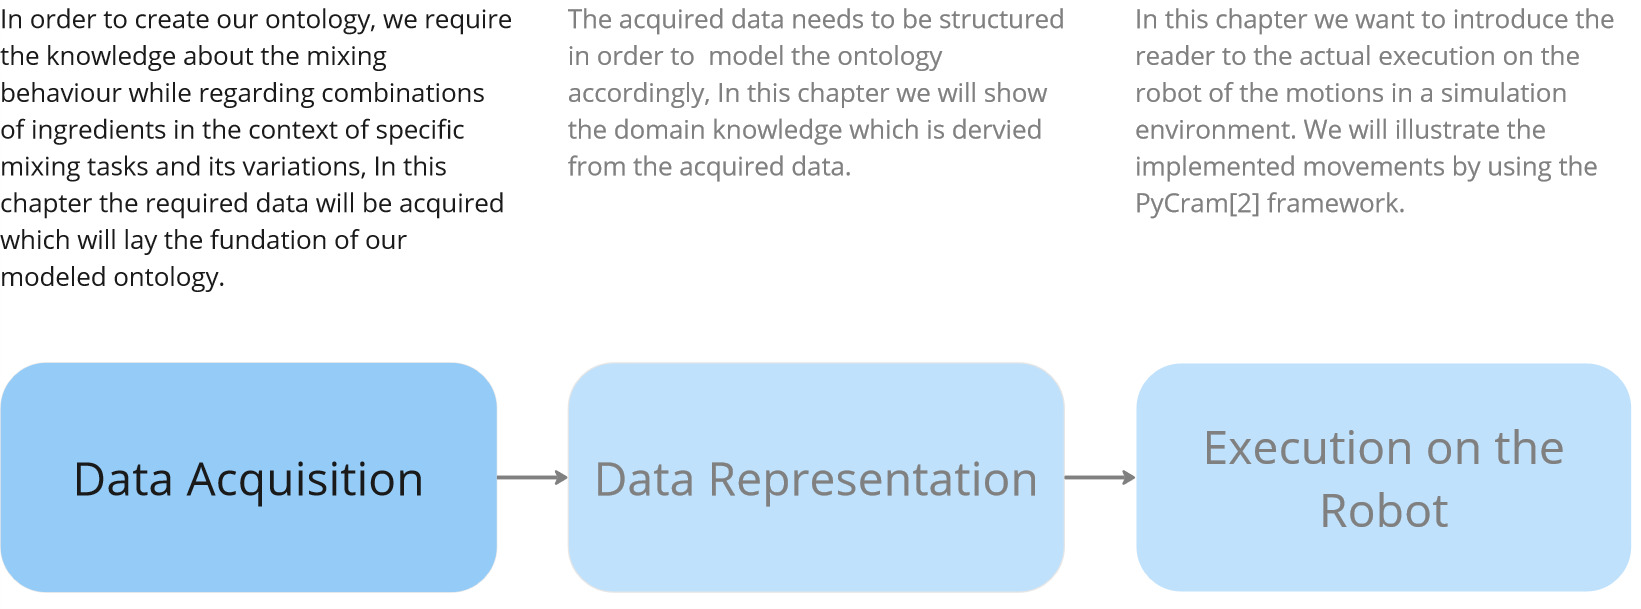
\includegraphics[scale=0.25]{Graphics/structure_overview1.jpg}
\end{figure}
Data acquisition involves understanding what mixing is, how it is performed by people, and how connections can be derived from video analyses. Essentially, it’s about discovering the various ways mixing is done, the contexts in which it occurs, and what insights we can draw from it. This includes identifying different mixing motions, determining which contexts are relevant, and which can be disregarded.
First we have to ask ourselves for our context \textbf{What is Mixing?}
\paragraph*{What is Mixing?}
  The definition provided by the Oxford Dictionary \cite{Oxford} is as follows:
  
  \textbf{Definition:} To put together or combine (two or more substances or things) so that the constituents or particles of each are interspersed or diffused more or less evenly among those of the rest; to unite (one or more substances or things) in this manner with another or others; to make a mixture of, to mingle, blend.

  Ultimately, this definition conveys that mixing requires at least two elements or substances, which are then combined (evenly) with each other, resulting in a (new) substance.
  This definition is general and can be applied to various contexts. For our work, the aspect of cooking or mixing different (cooking) ingredients is important. Therefore, we consider some hyponyms of the verb \textit{mixing} irrelevant for our cause and do not take them into account.
  An adapted definition for our work could be: 
  
  \textbf{Definition:} Mixing is the combination of various (cooking) ingredients through different motions in a container.
  

\section{Task variations}
Now that we have defined what \textit{mixing} means in our context, we aim to identify the various types of \textit{mixing} and determine which ones are important for our work. We will also specify which types of \textit{mixing} we will not consider further, providing arguments for our decisions.
	As our main focus is to represent the knowledge about mixing, first we had to acquire the different types and variations of mixing in order to create a complete Knowldegerepresentation. The first step in acquiring the needed data, was to acknowledge which task varations of mixing are actually important. 
  So we had to analyze the word \textit{Mixing} and its hyponyms. 
\subsection{Hyponyms} 
	Hyponyms are subordered words of a given word, for example one hyponym of \textit{mixing} could be \textit{beating}\cite{oxford_hyponym}.
  To conduct this analysis, one can utilize tools from various websites, such as FrameNet\cite{FrameNet} and WordNet\cite{WordNet}. These platforms provide users with the ability to search for specific words and obtain various associations for those words, including synonyms, acronyms, or, crucial for our case, hyponyms.	
  A full list of the considered hyponyms can be seen in table \ref{tab:hyponyms}.
\subsubsection{WikiHow Extraction}
  For all those hyponyms, we delegated a \textit{WikiHow} extraction search (see: \nameref{sec:WikiHow}) which should show us, how many times one of these words occur, in the context of cooking.
	To execute the search, we define a new Class \textit{MixingVerb}, which represents the verb \textit{mixing} and its hyponyms.
  
  For the search, we consider each verb and a triple consisting of the verb forms. We consider three forms of the verbs: the infinitive, the past tense, and the present progressive. An example of such a search would be:
  \begin{lstlisting}
      MIX ("mix", "mixed", "mixing")
  \end{lstlisting}

    After we have defined the desired verbs that we ultimately want to search for, we want to adjust some search parameters. The crucial parameters involve filtering the categories; in our case, we want to focus on mixing in the cooking domain. Therefore, we filter out all articles that do not exist in the \textit{Food and Entertaining} category.
  \subsubsection{Hyponyms Occurance}
    For each defined verb, a search is initiated to determine how often this verb appears in the \textit{WikiHow} articles \cite{wikihow}. This is done to ascertain which verbs are ultimately relevant for our implementation and which ones we can exclude, as they are infrequently used in everyday language.
    In the table below the results can be seen.
    \begin{table}[H]
        \centering
        \begin{tabular}{|c|c|}
          \hline
          \textbf{Hyponym} & \textbf{Occurance}  \\
          \hline
          Mix & 5300 \\
          \hline
          Amalgamate & 0 \\
          \hline
          Beat & 956 \\
          \hline
          Blend & 1041 \\
          \hline
          Coalesce & 1 \\
          \hline
          Combining & 3591  \\
          \hline
          Coommingle & 0 \\
          \hline
          Compound & 0 \\
          \hline
          Conflate & 0 \\
          \hline
          Folding & 821 \\
          \hline
          Fuse & 17 \\
          \hline
          Intermix & 0 \\
          \hline
          Join & 53 \\
          \hline
          Jumble & 0 \\
          \hline
          Lump & 7 \\
          \hline
          Merge & 6 \\
          \hline
          Pair & 352 \\
          \hline
          Stir & 6027 \\
          \hline
          Unify & 2 \\
          \hline
          Unite & 2 \\
          \hline
          Whip & 863 \\
          \hline
          Whisk & 2267 \\
          \hline
          
    
        \end{tabular}
        \caption{\textit{Mix}-verb synoyms/hyponyms occurance}
        \label{tab:hyponyms}
      \end{table}
      
  \subsubsection{Further Examination and Conclusion}
  This search is ultimately intended to provide us with information on which tasks we want to represent in the knowledge base. Therefore, we decide on certain tasks based on two conditions: frequency and executability. The first condition is easy to understand; tasks that do not occur or occur very rarely are not considered. The second condition relates to the executability of the task in the context of robot movements. Additionally, some tasks with relatively high frequency are also examined more closely, as in English, the past tense is used as an adjective under certain circumstances.

Taking into account the first condition, the following tasks are not considered: \textit{Amalgamate, Coalesce, Comingle, Compound, Conflate, Fuse, Intermix, Join, Jumble, Lump, Merge, Unify, and Unite}.

The second condition excludes another task: \textit{Blend. Blend} is mostly used in the context of a blending machine, which is not handled by the robot. Without this machine, the blending execution cannot be performed correctly, so this task is excluded for us.

Upon closer examination, we will also not consider the verb \textit{Whip} because it is mostly used as an adjective for ingredients, such as whipped cream. This highlights that only the verb \textit{Whip} has relatively low frequency. The same applies to \textit{Pair}, where the past tense is used to describe a combination of different ingredients, such as wine paired with cheese.

The verb \textit{combine} is not informative regarding the executed movement of an action and is equated to the verb  \textit{mix}.

Thus, the tasks we consider are: \textit{Mix, Beat, Fold, Stir, and Whisk.}

\section{Task Analysis and Defintion}
Now that we have selected the tasks, they need to be analyzed to understand the context in which they are ultimately used. 
Our goal is for the robot to perform these tasks in a manner similar to how a human would. 
To achieve this, in the next step, we need to closely examine these tasks. 
It is recommended to analyze videos on \textit{WikiHow} \cite{wikihow} or other sources where these tasks are presented as activities. 
The analysis involves observing the movements associated with each task. 
We present these analyses in tabular form below. The examination includes the task itself, the respective ingredients being processed, the tools used for it, and the container in which the task is carried out.
The tasks will be ennumerated, and we will provide the full table with the actual video source in the appendix (HERE REFERENCE TO APPENDIX).
    \begin{table}[H]
    \centering
    \begin{tabular}{|c|p{5,5cm}|p{6,5cm}|}
        \hline
        \textbf{Task} &  \textbf{Ingredients} & \textbf{Description} \\
        \hline
        Beating &  Egg yolk & circular, swirling wildly around the bowl \\
        \hline
        Stirring & Beaten Egg Yolk , Parmesan and Pepper  & Circular, from the inside to the outside. \\
        \hline
        Whisk & Eggs  & Circular but also straight, wildly motion. \\
        \hline
        Mixing &  Eggs, melted butter & Circular, from the inside to the outside, also diving. \\
        \hline
        Folding & cooked eggs in melted butter & Gently motion from the outisde to the inside straight, then moving about 90 degree before going to the inside again. \\
        \hline
      \end{tabular}
    \caption{Video analysis}
    \label{tab:videoanalysis}
  \end{table}


After a thorough analysis of the videos and the information provided in them, we conclude that the executed movement is not only related to the task but also influenced by the ingredients used. However, some tasks are deterministic in the sense that the movement is performed regardless of the specific ingredients.

In the following, we aim to structure the extracted information from the videos and present our findings.

\subsection{Video Analysis Conclusion and Results}

Based on the extracted information, we conclude that for our goals, the following aspects, in addition to the task, are important and will be further considered:
\begin{itemize}
  \item Ingredients: The ingredients play a crucial role in the movement decision associated with the tasks and will be defined more precisely.
  \item Tools: The tools used may not be decisive in the movement decision. Since we do not consider electric tools, every motion can be performed with any tool.
  \item Container: As conducted with the tools, the container wont play a crucial in the motion decision. 
  \item Motions: The motions ultimately represent the movement of the robot for our implementation. These movements are extracted from the videos and defined in alignment with robot motions.
\end{itemize}

\subsubsection{Ingredients}
Through the video analysis , we come to the conclusion that the nature of ingredients is important. 
Primarily, ingredients can be divided into two main categories: \textit{Dry} and \textit{Wet} \cite{Ohene2017}. 
This division becomes crucial, especially regarding the measurement of quantities for each type of ingredient.

For our case, a somewhat finer categorization of ingredients is necessary to map the various movements sensibly to the given types. 
In addition to \textit{Wet} ingredients, we introduce 2 new sub-categories: \textit{Liquid} and \textit{Semi-Liquid} ingredients. 
This corresponds to ingredients falling under the \textit{Wet} ingredients but with a liquid or semi-liquid state, such as milk, water, eggs, butter and oil. 
This is significant because some movements differ when the given ingredients are \textit{Semi-Liquid} or \textit{Liquid}.

We will also include 2 sub-categories for the \textit{Dry} category, namely the \textit{Solid} and \textit{Powder} ingredients category. 
This differs from the each other in that it consists of solid components, while we define the \textit{Powder} category to include powdery substances. The \textit{Solid} category encompasses foods like vegetables, fruits, and meats. 
Through these distinctions, we can create a definition refining the ingredient categories.

Our initial set of ingredients is: \textit{Milk, Oil, Water, Vinegar, Vanilla Extract, Sauces}, \textit{Egg White, Egg yolk, Butter, Whipped Cream}, \textit{Flour, Salt, Sugar, Baking Soda, Cocoa Powder},
\textit{Onions, Pork, Chicken, Minced meat, Bacon}.

These ingredients are commonly used in the analyzed videos and are also very common ingredients for baking and cooking recipes.
In the chapter \nameref{chap:Data_representation} these classes will be categorized.

\subsubsection{Containers and Tools}
\label{sec:ContainersAndToolsAcquisition}
Throughout the analysis of \textit{WikiHow} videos common tools and containers were identied during mixing task execution.
The most dominant occuring container was a bowl, followed by a pan, cup and then lastly a mug. Some common tools were used, like a whisk, spoon, spatula and mixer.
Since all of the containers can be used to serve or store food, this can be summarised in a single concept - crockery. \textbf{Crockery} is a concept in the \textit{SOMA-Home} \cite{soma}
ontology, by subsuming all of the subclasses of \textbf{Crockery}, we acquire in an instant many containers for mixing. Identified tools are partially represented by \textit{SOMA-Home},
mainly cutleries like spoons are belonging to this concept. Using \textbf{Cutlery} we can acquire a set of tools for mixing. Tools like whisks and mixers neither belong 
to the \textbf{Cutlery} concept nor have a representation in \textit{SOMA}, thus a higher level concept can't be acquired for these tools, to retrieve a set of tools resembling
kitchen tools.   


\subsubsection{Motions}
	From this videos we extracted informations about the executed motions. A detailled explanation of the motion can be found in the \nameref{chap:Motions} chapter. The following motions can be defined:
	\begin{itemize}
		\item \textbf{Circular}: Moving the tool in a defined circular movement in the container
		\item \textbf{Whirlstorm}: Moving from the inside to the outside of the container with the tool, like a whirlstorm.
		\item \textbf{Folding}: The folding motion in mixing involves lifting part of the material and folding it over the rest. This action helps blend the ingredients thoroughly. By repeating this motion, it will be ensured that everything is mixed evenly. It's a controlled and gentle way to combine ingredients.
		\item \textbf{Horizontal Eliptic}: We draw circles along a horizontal axis, trying to cover the entire container. This would look like covering the whole container from a bird's-eye view. This motion is commonly used by the beating task.
		\item \textbf{Circular Diving To Inner}: Starting from the outerside, moving the tool in the container arround its edge for about 3/4 of its circumference, before diving to the middle of the container. This motion is used by certain tasks where is required to turn the ingredients over.
	\end{itemize}

\section{Data Acquision Conclusion}

In the data acquisition phase, our focus was on creating a foundation of the necessary data and information required for a robot to perform various mixing tasks. After identifying the tasks, we were able to analyze videos to examine the movements associated with each task. We concluded that not only the task itself but also the selection of ingredients is crucial for determining the movement.

The ingredients are divided into four different categories, and we were able to define five motions that the robot should perform in a manner consistent with everyday use. In the next chapter, we will present how we intend to represent this knowledge and create a system that enables the robot to know which movement to execute based on a given task and set of ingredients.
\newpage